\documentclass[tikz, border=10pt]{standalone}
\usepackage{iftex}
\ifluatex
  \usepackage{fontspec}
  \usepackage{unicode-math}
  \setmainfont{Fira Sans}
  \setmonofont{Fira Mono}
  \setmathfont{Fira Math}
  \setmathfont{STIX Two Math}[range={"29F5,"2216}]
\else
  \usepackage[T1]{fontenc}
\fi

\usepackage{amsmath}
\usepackage{tikz}
\usetikzlibrary{arrows.meta}
\tikzset{every node/.style={font=\Large}}

% Theme toggle: \darkbgfalse for light background preview.
\newif\ifdarkbg
\darkbgfalse
\ifdarkbg
  \colorlet{axiscol}{white}
  \colorlet{gridcol}{white!30!black}
  \colorlet{ticklabelcol}{white}
  \colorlet{funcol}{yellow!85!white}
  \colorlet{auxcol}{white!50!black}
\else
  \colorlet{axiscol}{black}
  \colorlet{gridcol}{black!25!white}
  \colorlet{ticklabelcol}{black}
  \colorlet{funcol}{blue!70!black}
  \colorlet{auxcol}{black!40!white}
\fi

% x: -3 to 5   (8 units)   xscale=0.85 → ~6.8 cm wide
% y: -4 to 6  (10 units)   yscale=0.65 → ~6.5 cm tall  (square)
% Asymptotes: x=1 (vertical), y=1 (horizontal).
% Center of hyperbola: (1, 1).
% Clean integer points: (-1,0)  (0,-1)  (2,3)  (3,2)
\begin{document}
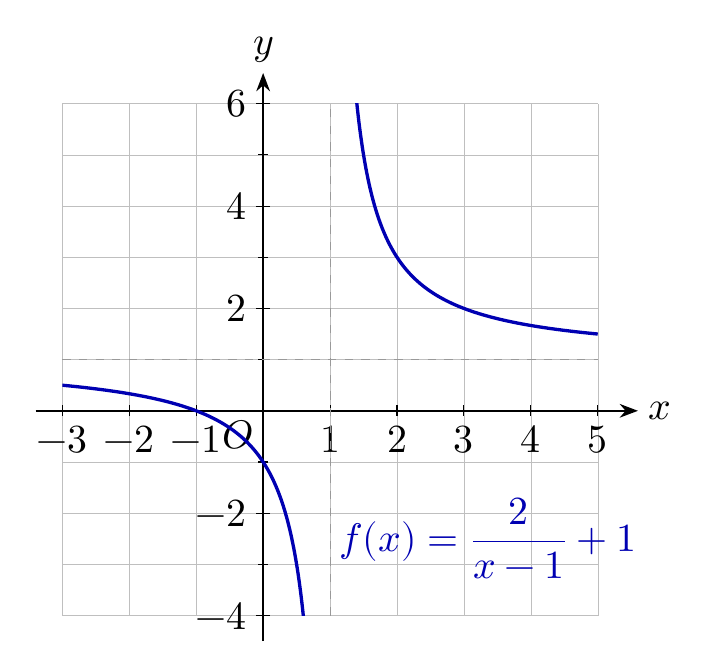
\begin{tikzpicture}[xscale=0.85, yscale=0.65, >=Stealth]

  % Cartesian grid.
  \draw[step=1, very thin, gridcol] (-3,-4) grid (5,6);

  % Axes.
  \draw[->, thick, axiscol] (-3.4,0) -- (5.6,0)
    node[right, text=axiscol] {$x$};
  \draw[->, thick, axiscol] (0,-4.5) -- (0,6.6)
    node[above, text=axiscol] {$y$};

  % Tick marks — x axis.
  \foreach \x in {-3,-2,-1,1,2,3,4,5} {
    \draw[axiscol] (\x, 3pt) -- (\x, -3pt)
      node[below, text=ticklabelcol] {$\x$};
  }

  % Tick marks — y axis (labelled every 2, minor every 1).
  \foreach \y in {-4,-2,2,4,6} {
    \draw[axiscol] (3pt,\y) -- (-3pt,\y)
      node[left, text=ticklabelcol] {$\y$};
  }
  \foreach \y in {-3,-1,1,3,5} {
    \draw[axiscol] (2pt,\y) -- (-2pt,\y);
  }

  % Origin label.
  \node[below left, text=axiscol] at (0,0) {$O$};

  % Asymptotes (dashed).
  \draw[dashed, auxcol] (1,-4)  -- (1,6);   % vertical:   x = 1
  \draw[dashed, auxcol] (-3,1)  -- (5,1);   % horizontal: y = 1

  % Function curves — two branches, clipped to window.
  \begin{scope}
    \clip (-3,-4) rectangle (5,6);
    % Left branch: x < 1
    \draw[domain=-3:0.97, smooth, very thick, funcol, samples=80]
      plot (\x, {2/(\x-1) + 1});
    % Right branch: x > 1
    \draw[domain=1.03:5, smooth, very thick, funcol, samples=80]
      plot (\x, {2/(\x-1) + 1});
  \end{scope}

  % Function label — upper-left, above the left branch.
  \node[right, text=funcol] at (1,-2.5) {$f(x)=\dfrac{2}{x-1}+1$};

  % Key points.
  % \node[circle, fill=funcol, inner sep=2pt] at (-1,0)  {};  % x-intercept
  % \node[circle, fill=funcol, inner sep=2pt] at (0,-1)  {};  % y-intercept
  % \node[circle, fill=funcol, inner sep=2pt] at (2,3)   {};
  % \node[circle, fill=funcol, inner sep=2pt] at (3,2)   {};

\end{tikzpicture}
\end{document}
